\graphicspath{ {images/} }

\titledquestion{Analyzing NMT Systems}[25]

\begin{parts}

    \part[3] Look at the {\monofam{src.vocab}} file for some examples of phrases and words in the source language vocabulary. When encoding an input Mandarin Chinese sequence into ``pieces'' in the vocabulary, the tokenizer maps the sequence to a series of vocabulary items, each consisting of one or more characters (thanks to the {\monofam{sentencepiece}} tokenizer, we can perform this segmentation even when the original text has no white space). Given this information, how could adding a 1D Convolutional layer after the embedding layer and before passing the embeddings into the bidirectional encoder help our NMT system? \textbf{Hint:} each Mandarin Chinese character is either an entire word or a morpheme in a word. Look up the meanings of 电, 脑, and 电脑 separately for an example. The characters 电 (electricity) and  脑 (brain) when combined into the phrase 电脑 mean computer.

            
    {\color{red}Solutions:

    在嵌入层之后添加一个一维的卷积层有助于每个窗口的词嵌入，帮助模型更好地理解上下文信息。
    滑动一个卷积过滤器能够帮助模型理解前后n个单词之间的关系，如果只看一个字或者一个词可能无法准确理解它在句子中的含义。
    
    }


    \part[8] Here we present a series of errors we found in the outputs of our NMT model (which is the same as the one you just trained). For each example of a reference (i.e., `gold') English translation, and NMT (i.e., `model') English translation, please:
    
    \begin{enumerate}
        \item Identify the error in the NMT translation.
        \item Provide possible reason(s) why the model may have made the error (either due to a specific linguistic construct or a specific model limitation).
        \item Describe one possible way we might alter the NMT system to fix the observed error. There are more than one possible fixes for an error. For example, it could be tweaking the size of the hidden layers or changing the attention mechanism.
    \end{enumerate}
    
    Below are the translations that you should analyze as described above. Only analyze the underlined error in each sentence. Rest assured that you don't need to know Mandarin to answer these questions. You just need to know English! If, however, you would like some additional color on the source sentences, feel free to use a resource like \url{https://www.archchinese.com/chinese_english_dictionary.html} to look up words. Feel free to search the training data file to have a better sense of how often certain characters occur.

    \begin{subparts}
        \subpart[2]
        \textbf{Source Sentence:} 贼人其后被警方拘捕及被判处盗窃罪名成立。 \newline
        \textbf{Reference Translation:} \textit{\underline{the culprits were} subsequently arrested and convicted.}\newline
        \textbf{NMT Translation:} \textit{\underline{the culprit was} subsequently arrested and sentenced to theft.}
        
        {\color{red}Solutions:
        
        贼人翻译成英语应该是复数形式，而不应该是单数形式。

        贼人既可以表示成单个人，也可以表示成一群人，在该句子中因为缺少了上下文信息，所以模型难以判断到底是一个人还是一群人。

        需要添加额外的上下文信息才能让模型判断出贼人代表的是一个人还是一群人。
        }

        \subpart[2]
        \textbf{Source Sentence}: 几乎已经没有地方容纳这些人,资源已经用尽。\newline
        \textbf{Reference Translation}: \textit{there is almost no space to accommodate these people, and resources have run out.   }\newline
        \textbf{NMT Translation}: \textit{the resources have been exhausted and \underline{resources have been exhausted}.}
        
        {\color{red}Solutions:
        
        NMT只翻译了“资源已经用尽”，而且翻译了两遍。

        原句中的两句话含义非常类似，模型可能并没有注意到正确的位置，使得模型只关注了最后一小段话的翻译，而忽略了前一段话的翻译。

        需要对模型的架构进行调整，并且添加更多地训练数据对模型进行训练，使其能够更好地进行生成操作。
        }

        \subpart[2]
        \textbf{Source Sentence}: 当局已经宣布今天是国殇日。 \newline
        \textbf{Reference Translation}: \textit{authorities have announced \underline{a national mourning today.}}\newline
        \textbf{NMT Translation}: \textit{the administration has announced \underline{today's day.}}
        
        {\color{red}Solutions:
        
        在模型翻译时漏掉了“国殇”的意思。

        在训练时，语料库可能缺少了对于“国殇”一词的出现，或者出现次数极少，使得模型没有学会对于“国殇”的翻译。

        需要在训练时使用更大的语料库和更丰富的上下文信息，使模型能够去翻译出现频率不高的单词。
        }
        
        \subpart[2] 
        \textbf{Source Sentence\footnote{This is a Cantonese sentence! The data used in this assignment comes from GALE Phase 3, which is a compilation of news written in simplified Chinese from various sources scraped from the internet along with their translations. For more details, see \url{https://catalog.ldc.upenn.edu/LDC2017T02}. }:} 俗语有云:``唔做唔错"。\newline
        \textbf{Reference Translation:} \textit{\underline{`` act not, err not "}, so a saying goes.}\newline
        \textbf{NMT Translation:} \textit{as the saying goes, \underline{`` it's not wrong. "}}
        
        {\color{red}Solutions:
        
        模型只翻译了“唔做唔错”的后一半的意思，并且意思也没有翻译到位。

        谚语在训练的语料库中并不是经常出现，使得模型并没有学会谚语的语法结构和含义。

        在训练的语料库中加入更多的谚语，让模型学会对谚语的翻译，并且可以提供一个预训练的解码器，帮助模型翻译谚语。
        }

    \end{subparts}


    \part[14] BLEU score is the most commonly used automatic evaluation metric for NMT systems. It is usually calculated across the entire test set, but here we will consider BLEU defined for a single example.\footnote{This definition of sentence-level BLEU score matches the \texttt{sentence\_bleu()} function in the \texttt{nltk} Python package. Note that the NLTK function is sensitive to capitalization. In this question, all text is lowercased, so capitalization is irrelevant. \\ \url{http://www.nltk.org/api/nltk.translate.html\#nltk.translate.bleu_score.sentence_bleu}
    } 
    Suppose we have a source sentence $\bs$, a set of $k$ reference translations $\br_1,\dots,\br_k$, and a candidate translation $\bc$. To compute the BLEU score of $\bc$, we first compute the \textit{modified $n$-gram precision} $p_n$ of $\bc$, for each of $n=1,2,3,4$, where $n$ is the $n$ in \href{https://en.wikipedia.org/wiki/N-gram}{n-gram}:
    \begin{align}
        p_n = \frac{ \displaystyle \sum_{\text{ngram} \in \bc} \min \bigg( \max_{i=1,\dots,k} \text{Count}_{\br_i}(\text{ngram}), \enspace \text{Count}_{\bc}(\text{ngram}) \bigg) }{\displaystyle \sum_{\text{ngram}\in \bc} \text{Count}_{\bc}(\text{ngram})}
    \end{align}
     Here, for each of the $n$-grams that appear in the candidate translation $\bc$, we count the maximum number of times it appears in any one reference translation, capped by the number of times it appears in $\bc$ (this is the numerator). We divide this by the number of $n$-grams in $\bc$ (denominator). \newline 

    Next, we compute the \textit{brevity penalty} BP. Let $len(c)$ be the length of $\bc$ and let $len(r)$ be the length of the reference translation that is closest to $len(c)$ (in the case of two equally-close reference translation lengths, choose $len(r)$ as the shorter one). 
    \begin{align}
        BP = 
        \begin{cases}
            1 & \text{if } len(c) \ge len(r) \\
            \exp \big( 1 - \frac{len(r)}{len(c)} \big) & \text{otherwise}
        \end{cases}
    \end{align}
    Lastly, the BLEU score for candidate $\bc$ with respect to $\br_1,\dots,\br_k$ is:
    \begin{align}
        BLEU = BP \times \exp \Big( \sum_{n=1}^4 \lambda_n \log p_n \Big)
    \end{align}
    where $\lambda_1,\lambda_2,\lambda_3,\lambda_4$ are weights that sum to 1. The $\log$ here is natural log.
    \newline
    \begin{subparts}
        \subpart[5] Please consider this example: \newline
        Source Sentence $\bs$: \textbf{需要有充足和可预测的资源。} 
        \newline
        Reference Translation $\br_1$: \textit{resources have to be sufficient and they have to be predictable}
        \newline
        Reference Translation $\br_2$: \textit{adequate and predictable resources are required}
        
        NMT Translation $\bc_1$: there is a need for adequate and predictable resources
        
        NMT Translation $\bc_2$: resources be sufficient and predictable to
        
        Please compute the BLEU scores for $\bc_1$ and $\bc_2$. Let $\lambda_i=0.5$ for $i\in\{1,2\}$ and $\lambda_i=0$ for $i\in\{3,4\}$ (\textbf{this means we ignore 3-grams and 4-grams}, i.e., don't compute $p_3$ or $p_4$). When computing BLEU scores, show your work (i.e., show your computed values for $p_1$, $p_2$, $len(c)$, $len(r)$ and $BP$). Note that the BLEU scores can be expressed between 0 and 1 or between 0 and 100. The code is using the 0 to 100 scale while in this question we are using the \textbf{0 to 1} scale. Please round your responses to 3 decimal places. 
        \newline
        
        Which of the two NMT translations is considered the better translation according to the BLEU Score? Do you agree that it is the better translation?
        
        {\color{red}Solutions:
        
        对于$\br_{1}$：

        1-gram:{"resources", "have", "to", "be", "sufficient", "and", "they", "have", "to", "be", "predictable"}

        2-gram:{"resources have", "have to", "to be", "be sufficient", "sufficient and", "and they", "they have", "have to", "to be", "be predictable"}

        3-gram:{"resources have to", "have to be", "to be sufficient", "be sufficient and", "sufficient and they", "and they have", "they have to", "have to be", "to be predictable"}
        
        4-gram:{"resources have to be", "have to be sufficient", "to be sufficient and", "be sufficient and they", "sufficient and they have", "and they have to", "they have to be", "have to be predictable"}

        len($\br_{1}$)=11

        对于$\br_{2}$：

        1-gram:{"adequate", "and", "predictable", "resources", "are", "required"}

        2-gram:{"adequate and", "and predictable", "predictable resources", "resources are", "are required"}

        3-gram:{"adequate and predictable", "and predictable resources", "predictable resources are", "resources are required"}
        
        4-gram:{"adequate and predictable resources", "and predictable resources are", "predictable resources are required"}

        len($\br_{2}$)=6

        对于$\bc_{1}$：

        1-gram:{"there", "is", "a", "need", "for", "adequate", "and", "predictable", "resources"}

        2-gram:{"there is", "is a", "a need", "need for", "for adequate", "adequate and", "and predictable", "predictable resources"}

        3-gram:{"there is a", "is a need", "a need for", "need for adequate", "for adequate and", "adequate and predictable", "and predictable resources"}
        
        4-gram:{"there is a need", "is a need for", "a need for adequate", "need for adequate and", "for adequate and predictable", "adequate and predictable resources"}

        len($\bc_{1}$)=9

        \begin{align*}
            p_{1} &= \frac{0 + 0 + 0 + 0 + 0 + 1 + 1 + 1 + 1}{9} = \frac{4}{9} \\
            p_{2} &= \frac{0 + 0 + 0 + 0 + 0 + 1 + 1 + 1}{8} = \frac{3}{8} \\
            p_{3} &= \frac{0 + 0 + 0 + 0 + 0 + 1 + 0}{7} = \frac{1}{7} \\
            p_{4} &= \frac{0 + 0 + 0 + 0 + 0 + 1}{6} = \frac{1}{6}
        \end{align*}

        $$
            BP_{1} = \exp(1 - \frac{len(\br_{1})}{len(\bc_{1})}) = \exp(1 - \frac{11}{9}) = \exp(-\frac{2}{9})
        $$

        那么可以得到BLEU分数：

        $$
            BLEU = \exp(-\frac{2}{9}) \times \exp(0.5 \times \log{\frac{4}{9}} + 0.5 \times \log{\frac{3}{8}} + 0 \times \log{\frac{1}{7}} + 0 \times \log{\frac{1}{6}}) \approx 0.327
        $$

        对于$\bc_{2}$：

        1-gram:{"resources", "be", "sufficient", "and", "predictable", "to"}

        2-gram:{"resources be", "be sufficient", "sufficient and", "and predictable", "predictable to"}

        3-gram:{"resources be sufficient", "be sufficient and", "sufficient and predictable", "and predictable to"}
        
        4-gram:{"resources be sufficient and", "be sufficient and predictable", "sufficient and predictable to"}

        len($\bc_{2}$)=6

        \begin{align*}
            p_{1} &= \frac{1 + 1 + 1 + 1 + 1 + 1}{6} = 1 \\
            p_{2} &= \frac{0 + 1 + 1 + 1 + 0}{5} = \frac{3}{5} \\
            p_{3} &= \frac{0 + 1 + 0 + 0}{4} = \frac{1}{4} \\
            p_{4} &= \frac{0 + 0  + 0}{3} = 0
        \end{align*}

        由于$len(\br_{2})=len(\bc_{2})$，因此

        $$
            BP_{2} = 1
        $$

        那么可以得到BLEU分数：

        $$
            BLEU = 1 \times \exp(0.5 \times \log{1} + 0.5 \times \log{\frac{3}{5}} + 0 \times \log{\frac{1}{4}}) \approx 0.775
        $$

        $\bc_{2}$的BLEU分数更高，但$\bc_{1}$对于句子的翻译更加准确，比$\bc_{2}$翻译的意思更加完善。因为BLEU分数是包含n-gram的，因此更高的BLEU分数并不能代表翻译的质量更高。
        }
        
        \subpart[5] Our hard drive was corrupted and we lost Reference Translation $\br_1$. Please recompute BLEU scores for $\bc_1$ and $\bc_2$, this time with respect to $\br_2$ only. Which of the two NMT translations now receives the higher BLEU score? Do you agree that it is the better translation?
        
        {\color{red}Solutions:
        
        对于$\bc_{1}$：

        \begin{align*}
            p_{1} &= \frac{0 + 0 + 0 + 0 + 0 + 1 + 1 + 1 + 1}{9} = \frac{4}{9} \\
            p_{2} &= \frac{0 + 0 + 0 + 0 + 0 + 1 + 1 + 1}{8} = \frac{3}{8} \\
            p_{3} &= \frac{0 + 0 + 0 + 0 + 0 + 1 + 1}{7} = \frac{2}{7} \\
            p_{4} &= \frac{0 + 0 + 0 + 0 + 0 + 1}{6} = \frac{1}{6}
        \end{align*}

        因为$len(\bc_{1}) > len(\br_{2})$，

        $$
            BP_{1} = 1
        $$

        那么可以得到BLEU分数：

        $$
            BLEU = 1 \times \exp(0.5 \times \log{\frac{4}{9}} + 0.5 \times \log{\frac{3}{8}} + 0 \times \log{\frac{2}{7}} + 0 \times \log{\frac{1}{6}}) \approx 0.408
        $$

        对于$\bc_{2}$：

        \begin{align*}
            p_{1} &= \frac{1 + 0 + 0 + 1 + 1 + 0}{6} = \frac{1}{2} \\
            p_{2} &= \frac{0 + 0 + 0 + 1 + 0}{5} = \frac{1}{5} \\
            p_{3} &= 0 \\
            p_{4} &= 0
        \end{align*}

        因为$len(\bc_{1}) = len(\br_{2})$，

        $$
            BP_{1} = 1
        $$

        那么可以得到BLEU分数：

        $$
            BLEU = 1 \times \exp(0.5 \times \log{\frac{1}{2}} + 0.5 \times \log{\frac{1}{5}}) \approx 0.316
        $$

        在没有$\br_{1}$的情况下，$\bc_{1}$的BLEU分数比$\bc_{2}$的BLEU分数更高，因此在这种情况下$\bc_{1}$更优。
        }
        
        \subpart[2] Due to data availability, NMT systems are often evaluated with respect to only a single reference translation. Please explain (in a few sentences) why this may be problematic. In your explanation, discuss how the BLEU score metric assesses the quality of NMT translations when there are multiple reference transitions versus a single reference translation.
        
        {\color{red}Solutions:
        
        通过前两个问题来计算一次翻译的BLEU分数，发现BLEU分数很依赖于n-gram的覆盖率，只要n-gram下模型的翻译和标准翻译越接近的，BLEU分数相对就会越高，但通常情况下，一个句子可以有多种翻译方式，
        即便BLEU分数不高但每一种翻译方式都不能算错，如果只使用一个参考翻译，会导致其他翻译的方式的BLEU分数很低，甚至从人们的视角来看非常合理的翻译也会得到很低的BLEU分数。参考翻译的多样性会让这种问题缓解，
        使得模型的翻译更加合理和多样化。
        }
        
        \subpart[2] List two advantages and two disadvantages of BLEU, compared to human evaluation, as an evaluation metric for Machine Translation. 
        
        {\color{red}Solutions:
        
        优点：

        \begin{itemize}
            \item BLEU分数提供了一种方便计算、不依赖于某种语言的自动化评估NMT系统翻译好坏的方式。
            \item 作为一种非主观的评估方式，BLEU分数可以应用到不同系统和模型的评估当中去。
        \end{itemize}

        缺点：

        \begin{itemize}
            \item BLEU高度依赖于n-gram匹配，BLEU分数的高低一定程度上取决于NMT系统翻译的和参考翻译是否高度匹配，但这会影响某些模型的翻译效果，从人类理解的程度上来说可能是合理的，
            但其BLEU分数并不会特别高，BLEU分数不能准确反映翻译的准确性。
            \item BLEU的n-gram匹配中每一个窗口的权重都是一样的，但对于不同长度的翻译来说，可能会潜在的影响计算的平衡性，导致好模型的BLEU分数不高。
        \end{itemize}
        }
        
    \end{subparts}


    \part[4] \emph{Beam search} is often employed to improve the quality of machine translation systems. While you were training the model, beam search results for the same example sentence at different iterations were also recorded in TensorBoard, and accessible in the \emph{TEXT} tab (Fig \ref{fig:beam-search-diagnostics-tensorboard}).

    The recorded diagnostic information includes json documents with the following fields: \texttt{example\_source} (the source sentence tokens), \texttt{example\_target} (the ground truth target sentence tokens), and \texttt{hypotheses} (10 hypotheses corresponding to the search result with beam size 10). Note that a predicted translation is often called \emph{hypothesis} in the neural machine translation jargon.

    \begin{subparts}
        \subpart[2] Did the translation quality improve over the training iterations for the model? Give three examples of translations of the example sentence at iterations 200, 3000, and the last iteration to illustrate your answer. For each iteration, pick the first beam search hypothesis as an example:
        
        {\color{red}Solutions:
        
        原句是：“我还澄清了在该会议上提出的若干事项。”

        \begin{itemize}
            \item 迭代2000次：
            i would also like to thank the number of a number of a number of a number of a number of a number of issues.
            \item 迭代44000次：
            i have also clarified a number of matters put forward at the conference.
            \item 最终迭代结果：
            i have also clarified the number of matters raised at that meeting.
        \end{itemize}

        与“I was able to provide clarification on some of the matters which were raised at that meeting.”相比，迭代次数越多，翻译的准确性和效果越好。
        }
        
        
        \subpart[2] How do various hypotheses resulting from beam search qualitatively compare? Give three other examples of hypotheses proposed by beam search at the last iteration to illustrate your answer.
        
        {\color{red}Solutions:
        
        \begin{itemize}
            \item I have also clarified the number of matters put forward at that meeting.得到的分数是-4.77。
            \item I also have clarified a number of matters put forward at that meeting.得到的分数是-5.78。
            \item I also have clarification on a number of matters put forward at that meeting.得到的分数是-6.37。
        \end{itemize}

        不同的hypotheses会导致不一样的分数，但分数高的并不一定就是最好的翻译，分数低的也不一定就说明翻译的不正确。
        }
        
    \end{subparts}



    \begin{figure}
        \centering
        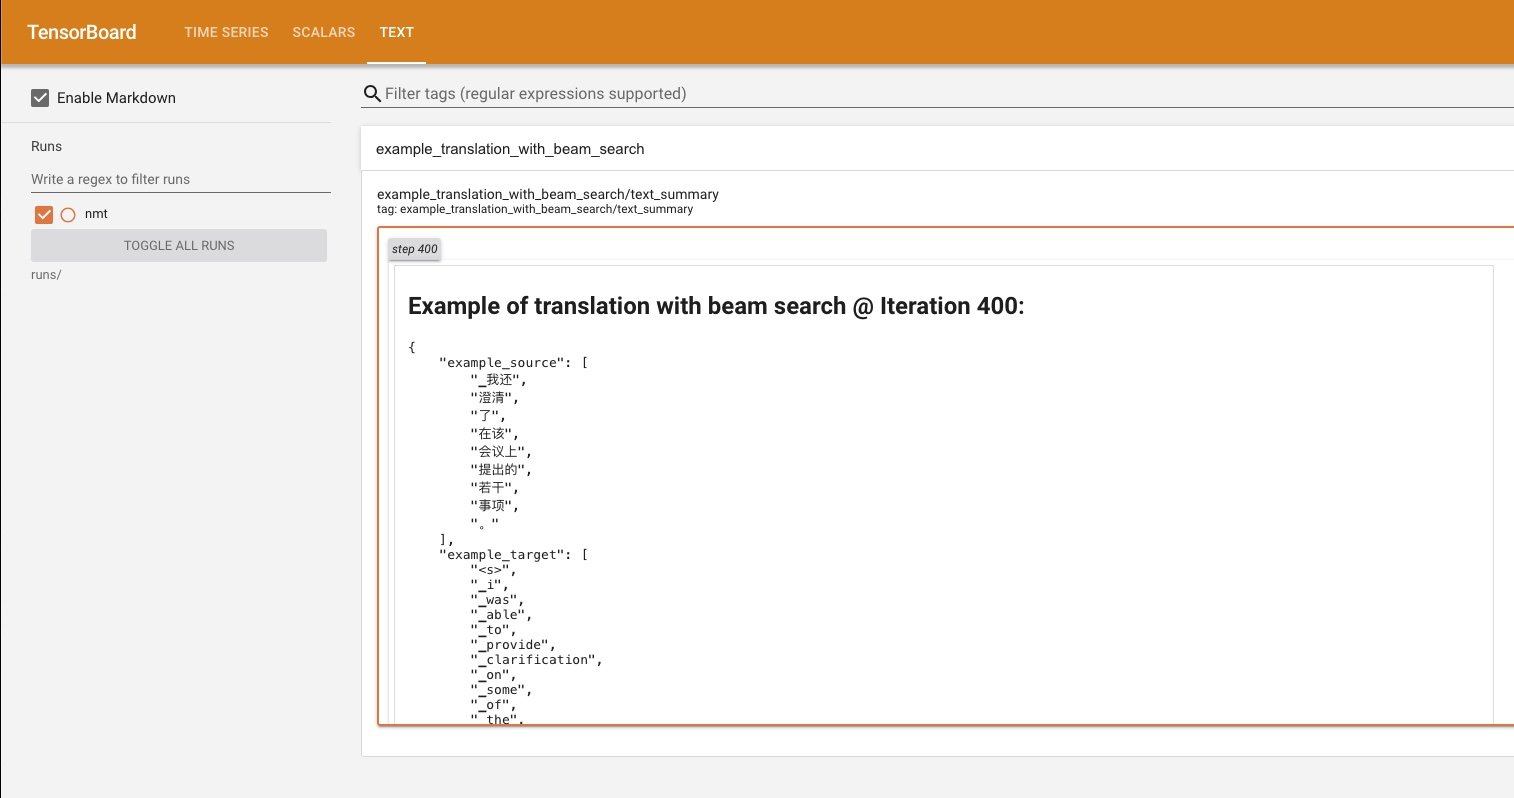
\includegraphics[width=0.7\textwidth]{images/example_translation_beam.jpg}
        \caption{Translation with beam search results for an example sentence are recorded in tensorboard for various iterations. The same data is available in the \texttt{outputs/beam\_search\_diagnostics/} folder in your working directory.}
        \label{fig:beam-search-diagnostics-tensorboard}
    \end{figure}
    

\end{parts}
